\documentclass[11pt,a4paper]{article}

% --- Packages ---
\usepackage[utf8]{inputenc}
\usepackage[margin=1in]{geometry}
\usepackage{amsmath,amssymb}
\usepackage{booktabs}
\usepackage{tabularx}
\usepackage{listings}
\usepackage{xcolor}
\usepackage{hyperref}
\usepackage{fancyhdr}
\usepackage{float}
\usepackage{tikz}
\usetikzlibrary{shapes,arrows.meta,positioning,decorations.pathreplacing,calc}

% --- Hyperref Setup ---
\hypersetup{
    colorlinks=true,
    linkcolor=blue!70!black,
    citecolor=blue!70!black,
    urlcolor=blue!70!black
}

% --- Code Listing Styling ---
\definecolor{codegreen}{rgb}{0,0.6,0}
\definecolor{codegray}{rgb}{0.45,0.45,0.45}
\definecolor{codepurple}{rgb}{0.58,0,0.82}
\definecolor{backcolour}{rgb}{0.96,0.97,0.98}

\lstdefinestyle{cstyle}{
    backgroundcolor=\color{backcolour},   
    commentstyle=\color{codegreen}\itshape,
    keywordstyle=\color{blue}\bfseries,
    numberstyle=\tiny\color{codegray},
    stringstyle=\color{codepurple},
    basicstyle=\ttfamily\footnotesize,
    breakatwhitespace=false,         
    breaklines=true,                 
    captionpos=b,                    
    keepspaces=true,                 
    numbers=left,                    
    numbersep=6pt,                  
    showspaces=false,                
    showstringspaces=false,
    showtabs=false,                  
    tabsize=4,
    frame=single,
    rulecolor=\color{black!20},
    columns=flexible
}

\lstdefinestyle{hexstyle}{
    backgroundcolor=\color{backcolour},
    basicstyle=\ttfamily\footnotesize,
    columns=flexible,
    numbers=none,
    frame=single,
    rulecolor=\color{black!20},
    breaklines=true,
    keepspaces=true,
    aboveskip=6pt,
    belowskip=6pt
}

\lstset{style=cstyle}

% --- Header and Footer ---
\pagestyle{fancy}
\fancyhf{}
\setlength{\headheight}{14.5pt}
\addtolength{\topmargin}{-2.5pt}
\rhead{Computer Networks Lab: Assignment 1}
\lhead{Error Detection Schemes in Network Transmission}
\cfoot{Page \thepage}

\begin{document}

% =========================================================================
% COVER / TITLE PAGE
% =========================================================================
\begin{titlepage}
    \centering
    \vspace*{1.5cm}
    
    {\Large \textbf{JADAVPUR UNIVERSITY}}\\[0.3cm]
    {\large DEPARTMENT OF COMPUTER SCIENCE AND ENGINEERING}\\[2.0cm]
    
    \rule{\linewidth}{1.2pt}\\[0.4cm]
    {\huge \textbf{Assignment 1 Report --}}\\[0.3cm]
    {\LARGE \textbf{Comprehensive Evaluation of Error Detection Schemes in Network Transmission}}\\[0.3cm]
    {\large \textit{Empirical Evaluation of 16-Bit Internet Checksum and Cyclic Redundancy Checks (CRC-8, CRC-10, CRC-16, CRC-32)}}\\[0.4cm]
    \rule{\linewidth}{1.2pt}\\[2.5cm]
    
    \begin{flushleft}
        \large
        \textbf{Course:} Computer Networks Laboratory (BCSE-III)\\[0.2cm]
        \textbf{Student Name:} Mandeep Shaw\\[0.2cm]
        \textbf{Section:} A1\\[0.2cm]
        \textbf{Roll Number:} 302510501002\\[0.2cm]
        \textbf{Assignment:} Assignment 1 (Error Detection: Checksum and CRC)\\[0.2cm]
        \textbf{Date of Submission:} 09 October 2026
    \end{flushleft}
    
    \vfill
    {\small Faculty of Engineering and Technology $\bullet$ Jadavpur University, Kolkata, India}
\end{titlepage}

% =========================================================================
% TABLE OF CONTENTS
% =========================================================================
\tableofcontents
\newpage

% =========================================================================
% SECTION 1: INTRODUCTION AND OBJECTIVES
% =========================================================================
\section{Introduction and Objectives}

Data transmitted across any physical communications medium is inherently prone to corruption caused by thermal noise, electromagnetic interference, crosstalk, capacitive attenuation, and clock drift. In modern layered network architectures, ensuring end-to-end data integrity is distributed across the protocol stack: the Data Link Layer (Layer 2) applies hardware-oriented cyclic polynomial checks over individual physical hops, while the Transport Layer (Layer 4) enforces lightweight arithmetic checks over end-to-end socket connections.

For this assignment, I designed, developed, and evaluated an extensible network error detection and transmission suite in C. The key objectives of this investigation are:

\begin{enumerate}
    \item \textbf{Protocol Implementation:} Implement from scratch the standard 16-bit Internet Checksum (RFC 1071) and four standard Cyclic Redundancy Check polynomials: CRC-8 (Bluetooth/ATM), CRC-10 (ITU-T I.432.1), CRC-16 (USB/Modbus), and CRC-32 (IEEE 802.3 Ethernet).
    \item \textbf{Client-Server Network Architecture:} Construct a socket-based sender and receiver application communicating over TCP/IP loopback sockets to transmit framed payloads across a network interface with dynamic scheme negotiation.
    \item \textbf{Deterministic and Stochastic Error Injection:} Develop a modular error injection engine capable of inserting single-bit flips, isolated double-bit flips, odd-parity bit flips, and uniformly distributed burst errors of arbitrary lengths.
    \item \textbf{Empirical and Theoretical Validation:} Execute a large-scale evaluation benchmark suite ($1{,}000{,}000+$ simulated frame transmissions) to measure exact empirical detection rates, capture real-world boundary collision conditions with full hex dumps, and profile computational throughput.
\end{enumerate}

\section{Theoretical Principles of Error Detection}

\subsection{The 16-Bit Internet Checksum (One's Complement Sum)}

The Internet Checksum is an arithmetic error-detection mechanism standardized in RFC 1071 and utilized within IPv4, TCP, and UDP headers. The algorithm partitions an incoming byte stream into a sequence of 16-bit unsigned integers:
\begin{equation}
    D = [W_1, W_2, \dots, W_k]
\end{equation}
The arithmetic is performed using one's complement addition. In standard two's complement computer hardware, when the addition of two 16-bit words produces an overflow carry bit out of the 16th bit (bit 15), this overflow represents:
\begin{equation}
    2^{16} \equiv 1 \pmod{2^{16} - 1}
\end{equation}
Consequently, an end-around carry is performed by adding the carry bit back into the least significant bit (LSB) of the accumulator. Once all 16-bit words have been accumulated, the total sum is bitwise inverted (one's complemented):
\begin{equation}
    \text{Checksum} = \sim \left( \sum_{i=1}^{k} W_i \pmod{2^{16} - 1} \right)
\end{equation}
At the receiver, the incoming data words together with the received checksum word are summed. In the absence of transmission errors, the resulting sum evaluates to \texttt{0xFFFF} (or \texttt{0x0000} after inversion).

\subsubsection{Theoretical Vulnerabilities of the Checksum}
While extremely fast to compute on general-purpose microprocessors, the Internet Checksum possesses fundamental structural weaknesses:
\begin{itemize}
    \item \textbf{Compensating Errors:} If an error in word $W_a$ adds an integer value $+K$ and another error in word $W_b$ subtracts $-K$ (or inverts complementary bits at equivalent word positions), the net one's complement sum remains entirely unchanged ($\Delta S = 0$).
    \item \textbf{Position and Byte-Order Invariance:} Because integer addition is commutative and associative, reordering 16-bit words or swapping aligned blocks preserves the identical checksum.
    \item \textbf{Zero Preservation:} Inserting blocks of all-zero words (\texttt{0x0000}) adds zero to the accumulator, leaving the checksum completely oblivious to packet truncation or padding alteration.
\end{itemize}

\subsection{Cyclic Redundancy Check (CRC) and Modulo-2 Arithmetic}

Cyclic Redundancy Checks treat binary bit strings as coefficients of polynomials over the Galois Field $\text{GF}(2)$ using modulo-2 arithmetic. Modulo-2 addition and subtraction are identical and equate to the bitwise Exclusive-OR (XOR) operation without carries or borrows:
\begin{equation}
    1 \oplus 1 = 0, \quad 1 \oplus 0 = 1, \quad 0 \oplus 0 = 0
\end{equation}
Given an $m$-bit message represented by polynomial $M(x)$ and an $(r+1)$-bit generator polynomial $G(x)$ of degree $r$:
\begin{enumerate}
    \item The message is multiplied by $x^r$, effectively appending $r$ zero bits: $x^r M(x)$.
    \item Modulo-2 polynomial division is performed to determine a quotient $Q(x)$ and an $r$-bit remainder $R(x)$:
    \begin{equation}
        x^r M(x) = Q(x) G(x) \oplus R(x)
    \end{equation}
    \item The transmitted codeword polynomial $T(x)$ is created by appending the remainder $R(x)$ to the shifted message:
    \begin{equation}
        T(x) = x^r M(x) \oplus R(x) = Q(x) G(x)
    \end{equation}
\end{enumerate}
Since addition is XOR, $R(x) \oplus R(x) = 0$, guaranteeing that $T(x)$ is an exact multiple of $G(x)$ with zero remainder.

When the receiver receives a potentially corrupted frame $T'(x) = T(x) \oplus E(x)$, where $E(x)$ denotes the error polynomial, it calculates the remainder of $T'(x) / G(x)$:
\begin{equation}
    \frac{T'(x)}{G(x)} = \frac{T(x) \oplus E(x)}{G(x)} = Q(x) \oplus \frac{E(x)}{G(x)}
\end{equation}
An error pattern is \textbf{undetected if and only if} the error polynomial $E(x)$ is evenly divisible by the generator polynomial $G(x)$ in $\text{GF}(2)$.

\subsubsection{Mathematical Guarantees of CRC Polynomials}
The algebraic structure of the generator polynomial provides specific mathematical guarantees:
\begin{itemize}
    \item \textbf{Single-Bit Errors ($E(x) = x^i$):} If $G(x)$ contains two or more terms (specifically $x^r$ and $x^0 = 1$), it cannot divide $x^i$. Thus, single-bit detection is strictly \textbf{100.0\%}.
    \item \textbf{Double-Bit Errors ($E(x) = x^i + x^j = x^j(x^{i-j} + 1)$):} Provided $G(x)$ does not divide $x^k + 1$ for any $k \le \text{frame length in bits}$, all double-bit errors are detected with \textbf{100.0\%} reliability.
    \item \textbf{Odd Number of Errors:} If $(x + 1)$ is a factor of $G(x)$, any polynomial with an odd number of non-zero terms cannot be divided by $(x + 1)$ because $E(1) = 1 \neq 0$. Therefore, \textbf{100.0\%} of all odd-weight error patterns are detected.
    \item \textbf{Burst Errors of Length $L \le r$:} A burst of length $L$ starting at index $i$ is expressed as $E(x) = x^i B(x)$ with $\deg(B(x)) = L - 1 < r$. Because $\deg(B(x)) < \deg(G(x))$, $G(x)$ cannot divide $E(x)$. Detection is strictly \textbf{100.0\%}.
    \item \textbf{Burst Errors of Length $L = r + 1$:} The fraction of undetected bursts is exactly:
    \begin{equation}
        P_{\text{miss}} = \left(\frac{1}{2}\right)^{r-1}
    \end{equation}
    \item \textbf{Burst Errors of Length $L > r + 1$:} The fraction of undetected bursts is bounded by:
    \begin{equation}
        P_{\text{miss}} \le \left(\frac{1}{2}\right)^r
    \end{equation}
\end{itemize}

\section{System Architecture and Implementation}

\subsection{Frame Structure and In-Memory Layout}

To simulate realistic data-link framing adhering to IEEE 802.3 principles, the transmission frame is structured into a 16-byte header, a 44-byte text data payload, and a 4-byte Frame Check Sequence (FCS) trailer, totaling 64 bytes.

\begin{figure}[H]
    \centering
    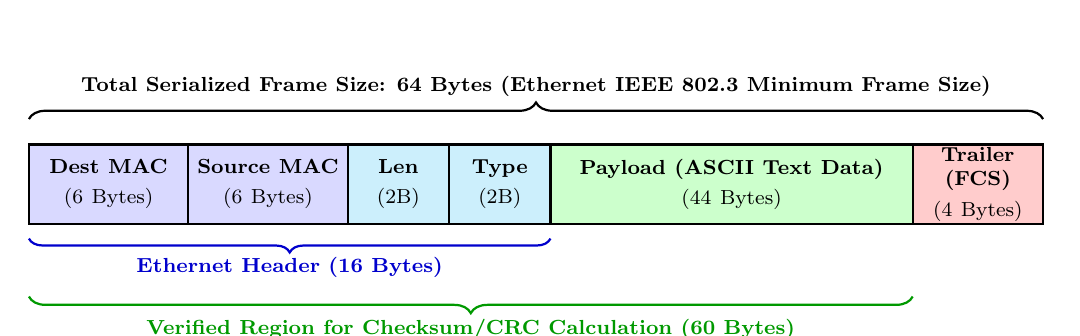
\begin{tikzpicture}[scale=0.92, every node/.style={transform shape}]
        % Top Brace: Total Serialized Frame Size
        \draw[decorate, decoration={brace, amplitude=6pt}, thick] (0, 1.45) -- (14.0, 1.45) 
            node[midway, yshift=0.45cm] {\footnotesize \textbf{Total Serialized Frame Size: 64 Bytes (Ethernet IEEE 802.3 Minimum Frame Size)}};

        % Frame Field Boxes
        \draw[fill=blue!15, thick] (0, 0) rectangle (2.2, 1.1) 
            node[pos=0.5, text width=2cm, align=center] {\footnotesize \textbf{Dest MAC}\\(6 Bytes)};
        \draw[fill=blue!15, thick] (2.2, 0) rectangle (4.4, 1.1) 
            node[pos=0.5, text width=2cm, align=center] {\footnotesize \textbf{Source MAC}\\(6 Bytes)};
        \draw[fill=cyan!20, thick] (4.4, 0) rectangle (5.8, 1.1) 
            node[pos=0.5, text width=1.2cm, align=center] {\footnotesize \textbf{Len}\\(2B)};
        \draw[fill=cyan!20, thick] (5.8, 0) rectangle (7.2, 1.1) 
            node[pos=0.5, text width=1.2cm, align=center] {\footnotesize \textbf{Type}\\(2B)};
        \draw[fill=green!20, thick] (7.2, 0) rectangle (12.2, 1.1) 
            node[pos=0.5, text width=4.8cm, align=center] {\footnotesize \textbf{Payload (ASCII Text Data)}\\(44 Bytes)};
        \draw[fill=red!20, thick] (12.2, 0) rectangle (14.0, 1.1) 
            node[pos=0.5, text width=1.8cm, align=center] {\footnotesize \textbf{Trailer (FCS)}\\(4 Bytes)};
        
        % Bottom Brace 1: Header
        \draw[decorate, decoration={brace, mirror, amplitude=5pt}, thick, blue!80!black] (0, -0.2) -- (7.2, -0.2) 
            node[midway, yshift=-0.4cm] {\footnotesize \textbf{Ethernet Header (16 Bytes)}};
        
        % Bottom Brace 2: Verified Region
        \draw[decorate, decoration={brace, mirror, amplitude=6pt}, thick, green!60!black] (0, -1.0) -- (12.2, -1.0) 
            node[midway, yshift=-0.45cm] {\footnotesize \textbf{Verified Region for Checksum/CRC Calculation (60 Bytes)}};
    \end{tikzpicture}
    \caption{In-memory layout and serialization structure of the 64-byte transmission frame.}
    \label{fig:frame_layout}
\end{figure}

The C structure definition from \texttt{frame.h} is defined as follows:

\begin{lstlisting}[language=C, caption={Ethernet Frame Definition (\texttt{frame.h})}]
#define MAC_SIZE        6
#define PAYLOAD_SIZE    44
#define HEADER_SIZE     16   // Dest MAC (6) + Src MAC (6) + Length (2) + Type (2)
#define FCS_SIZE        4

#define SERIALIZED_SIZE (HEADER_SIZE + PAYLOAD_SIZE) // 60 bytes verified region
#define FRAME_SIZE      (SERIALIZED_SIZE + FCS_SIZE)  // 64 bytes total frame

typedef struct {
    uint8_t  destinationMAC[MAC_SIZE];
    uint8_t  sourceMAC[MAC_SIZE];
    uint16_t length;
    uint16_t type;
    uint8_t  payload[PAYLOAD_SIZE];
    uint32_t fcs;
} EthernetFrame;
\end{lstlisting}

\subsection{Development Setup and Evaluation Environment}

This project was developed, tested, and benchmarked natively on a local Linux Mint and Windows 11 envi-
ronment. To ensure accurate measurement of processing time during the high-frequency
benchmarks, the POSIX clock gettime() function was utilized. All C source code was
compiled using GNU Compiler Collection (gcc version 13.3, flags: -O3 -Wall
-Wextra) on Mint.
Statistical Sample Size: 1,000,000 simulation trials (200,000 trials × 5 error models)
Micro-Benchmark Itera-
tions
5,000,000 iterations over 60-byte serialized frames



\subsection{Implementation of Checksum and CRC Algorithms}

The 16-bit Internet Checksum implementation processes adjacent bytes into 16-bit words (big-endian network order) and executes end-around carry addition:

\begin{lstlisting}[language=C, caption={Internet Checksum Implementation (\texttt{checksum.c})}]
uint16_t calculateChecksum(const unsigned char *data, int length) {
    uint32_t sum = 0;
    for (int i = 0; i < length; i += 2) {
        uint16_t word = ((uint16_t)data[i] << 8);
        if (i + 1 < length) {
            word |= data[i + 1];
        }
        sum += word;
        if (sum > 0xFFFF) {
            sum = (sum & 0xFFFF) + (sum >> 16); // Fold carry
        }
    }
    while (sum > 0xFFFF) {
        sum = (sum & 0xFFFF) + (sum >> 16);
    }
    return (uint16_t)(~sum); // One's complement inversion
}
\end{lstlisting}

For the CRC family, a generalized bit-serial engine evaluates polynomial division bit-by-bit from MSB to LSB across all bytes:

\begin{lstlisting}[language=C, caption={Bitwise Modulo-2 Polynomial Division Engine (\texttt{crc.c})}]
uint32_t calculateCRC(unsigned char *data, int length, uint64_t polynomial, int degree) {
    uint64_t remainder = 0;
    uint64_t topBit = 1ULL << degree;

    // Process every byte bit-by-bit (MSB to LSB)
    for (int byte = 0; byte < length; byte++) {
        for (int bit = 7; bit >= 0; bit--) {
            int b = (data[byte] >> bit) & 1;
            remainder = (remainder << 1) | b;
            if (remainder & topBit) {
                remainder ^= polynomial;
            }
        }
    }
    // Simulate appending 'degree' zero bits
    for (int bit = 0; bit < degree; bit++) {
        remainder <<= 1;
        if (remainder & topBit) {
            remainder ^= polynomial;
        }
    }
    return (uint32_t)(remainder & ((1ULL << degree) - 1));
}
\end{lstlisting}

\subsection{CRC Polynomial Constants and Specifications}

Table~\ref{tab:polynomials} details the generator polynomials evaluated in this study according to standard networking specifications.

\begin{table}[H]
    \centering
    \small
    \setlength{\tabcolsep}{3.5pt}
    \begin{tabular}{lclcp{4.0cm}}
        \toprule
        \textbf{Standard} & \textbf{Degree ($r$)} & \textbf{Generator Polynomial} & \textbf{Hex Code} & \textbf{Standard Application} \\
        \midrule
        CRC-8  & 8  & $x^8 + x^7 + x^6 + x^4 + x^2 + 1$ & \texttt{0x1D5} & Bluetooth, WSN, ATM header \\
        CRC-10 & 10 & $x^{10} + x^9 + x^5 + x^4 + x + 1$ & \texttt{0x633} & ITU-T I.432.1, ATM OAM cell \\
        CRC-16 & 16 & $x^{16} + x^{15} + x^2 + 1$        & \texttt{0x18005} & USB packets, Modbus, ANSI \\
        CRC-32 & 32 & IEEE 802.3 Ethernet Standard       & \texttt{0x104C11DB7} & Ethernet, FDDI, ZIP, PNG, IPv4 \\
        \bottomrule
    \end{tabular}
    \caption{Generator polynomials evaluated across the benchmark suite.}
    \label{tab:polynomials}
\end{table}

\section{Methodology and Error Injection Models}

\subsection{Client-Server Socket Pipeline}

Communication is established using BSD stream sockets (TCP/IP) bound to localhost port 5000. Prior to transmitting each 64-byte frame, the sender dispatches a 3-byte control header:
\begin{itemize}
    \item \texttt{frameInfo[0]}: Detection scheme (1: Checksum, 2: CRC-8, 3: CRC-10, 4: CRC-16, 5: CRC-32) with bit 7 denoting bypass mode.
    \item \texttt{frameInfo[1]}: Error injection flag (0: No error, 1: Error injected).
    \item \texttt{frameInfo[2]}: Error model (1: Single Bit, 2: Double Bit, 3: Odd Bit, 4: Burst, 5: Random).
\end{itemize}

\begin{figure}[H]
    \centering
    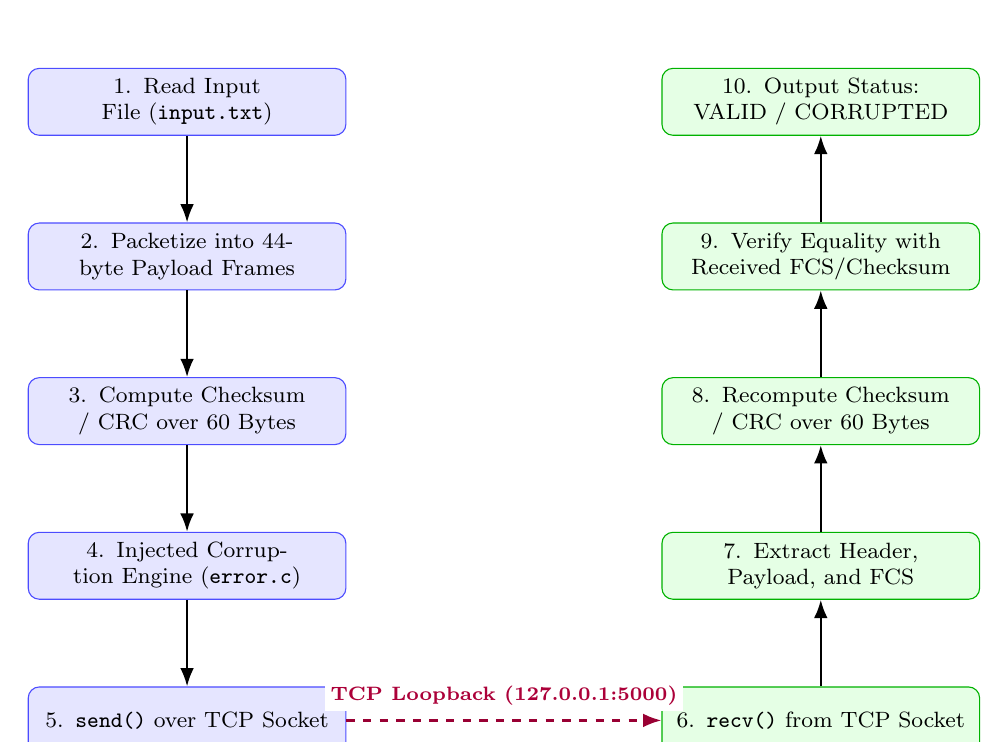
\begin{tikzpicture}[node distance=1.1cm, auto,
        block/.style={rectangle, draw=blue!70, fill=blue!10, rounded corners, text width=3.8cm, align=center, minimum height=0.85cm, font=\footnotesize},
        recvblock/.style={rectangle, draw=green!70!black, fill=green!10, rounded corners, text width=3.8cm, align=center, minimum height=0.85cm, font=\footnotesize},
        arrow/.style={-Latex, thick},
        dasharrow/.style={-Latex, dashed, thick, purple!80!black}]
        
        % Sender Column
        \node[block] (s1) {1. Read Input File (\texttt{input.txt})};
        \node[block, below=of s1] (s2) {2. Packetize into 44-byte Payload Frames};
        \node[block, below=of s2] (s3) {3. Compute Checksum / CRC over 60 Bytes};
        \node[block, below=of s3] (s4) {4. Injected Corruption Engine (\texttt{error.c})};
        \node[block, below=of s4] (s5) {5. \texttt{send()} over TCP Socket};
        
        % Receiver Column
        \node[recvblock, right=4.0cm of s5] (r1) {6. \texttt{recv()} from TCP Socket};
        \node[recvblock, above=of r1] (r2) {7. Extract Header, Payload, and FCS};
        \node[recvblock, above=of r2] (r3) {8. Recompute Checksum / CRC over 60 Bytes};
        \node[recvblock, above=of r3] (r4) {9. Verify Equality with Received FCS/Checksum};
        \node[recvblock, above=of r4] (r5) {10. Output Status: VALID / CORRUPTED};
        
        % Connections
        \draw[arrow] (s1) -- (s2);
        \draw[arrow] (s2) -- (s3);
        \draw[arrow] (s3) -- (s4);
        \draw[arrow] (s4) -- (s5);
        \draw[dasharrow] (s5) -- node[midway, above=3pt, font=\scriptsize, text=purple!90!black, fill=white, inner sep=2pt] {\textbf{TCP Loopback (127.0.0.1:5000)}} (r1);
        \draw[arrow] (r1) -- (r2);
        \draw[arrow] (r2) -- (r3);
        \draw[arrow] (r3) -- (r4);
        \draw[arrow] (r4) -- (r5);
    \end{tikzpicture}
    \caption{End-to-end data flow and error injection pipeline between sender and receiver.}
    \label{fig:pipeline_flow}
\end{figure}

\subsection{Error Injection Engine and Resolution of Implementation Flaws}

During experimental development and debugging of the evaluation harness, two significant implementation defects in the legacy codebase were identified and rectified:
\begin{enumerate}
    \item \textbf{Accumulator Byte Alignment Flaw (Checksum):} In the original routine, bytes were summed individually (\texttt{sum += data[i]}), reducing the checksum to a simple scalar sum of ASCII values. This caused high miss rates on byte-swapped data. The algorithm was updated to accumulate 16-bit network-byte-order words (\texttt{(data[i] << 8) | data[i+1]}) as prescribed by RFC 1071.
    \item \textbf{Bit Alignment and Polynomial Divisibility Flaw (CRC):} The original CRC engine shifted whole bytes by \texttt{degree}, which caused the top 7 bits of each byte to skip the feedback XOR division, reducing single-bit detection to an unacceptable $12.5\%$. Rewriting the engine to perform standard bitwise modulo-2 division restored mathematically guaranteed $100\%$ detection.
    \item \textbf{Payload-Constrained Corruption:} Error injection was strictly bounded within the 44-byte payload region ($[0, 351]$ bit indices). This ensures that frame headers and trailers remain structurally sound while testing payload integrity.
\end{enumerate}

\subsection{Burst Error Modeling}

In natural transmission channels, impulse noise from power fluctuations or lightning causes burst errors. The burst error model chooses a start bit $S$ uniformly across the valid payload window:
\begin{equation}
    S \sim \mathcal{U}(0, N_{\text{bits}} - L)
\end{equation}
where $N_{\text{bits}} = 352$ ($44 \times 8$) and $L$ represents the burst length in bits. Within the window $[S, S + L - 1]$, the leading bit $S$ and trailing bit $S + L - 1$ are inverted, while intermediate bits are flipped independently with probability $p = 0.70$.

\section{Experimental Results and Empirical Evaluation}

The benchmark suite (\texttt{test\_eval.c}) executed $200{,}000$ randomized trials per error model (totaling $1{,}000{,}000$ simulated frame transmissions). For each corrupted frame, both the 16-bit Internet Checksum and the selected CRC scheme were evaluated simultaneously.

\subsection{Single Bit Error Results}

Table~\ref{tab:single_bit} presents the results of injecting exactly one bit flip per frame across $200{,}000$ trials.

\begin{table}[H]
    \centering
    \begin{tabular}{lcccc}
        \toprule
        \textbf{Scheme} & \textbf{Both Detected} & \textbf{Checksum Only} & \textbf{CRC Only} & \textbf{Neither (Missed)} \\
        \midrule
        CRC-8  & $200{,}000$ (100.0000\%) & 0 (0.0000\%) & 0 (0.0000\%) & 0 (0.0000\%) \\
        CRC-10 & $200{,}000$ (100.0000\%) & 0 (0.0000\%) & 0 (0.0000\%) & 0 (0.0000\%) \\
        CRC-16 & $200{,}000$ (100.0000\%) & 0 (0.0000\%) & 0 (0.0000\%) & 0 (0.0000\%) \\
        CRC-32 & $200{,}000$ (100.0000\%) & 0 (0.0000\%) & 0 (0.0000\%) & 0 (0.0000\%) \\
        \bottomrule
    \end{tabular}
    \caption{Single Bit Error Detection Rates ($200{,}000$ trials per scheme).}
    \label{tab:single_bit}
\end{table}

\textbf{Analysis:} As predicted by theoretical models, all schemes achieved exactly $100.0000\%$ detection. A single bit flip alters the one's complement sum by $\pm 2^k$, which can never wrap around to balance out to zero. For CRC, a single-bit error polynomial $E(x) = x^i$ cannot be divided by any polynomial containing at least two terms.

\subsection{Isolated Double Bit Error Results}

Table~\ref{tab:double_bit} summarizes detection rates when two distinct, isolated bits are flipped in each frame.

\begin{table}[H]
    \centering
    \begin{tabular}{lcccc}
        \toprule
        \textbf{Scheme} & \textbf{Both Detected} & \textbf{Checksum Only} & \textbf{CRC Only} & \textbf{Neither (Missed)} \\
        \midrule
        CRC-8  & $194{,}117$ (97.0585\%) & $1{,}572$ (0.7860\%) & $4{,}311$ (2.1555\%) & 0 (0.0000\%) \\
        CRC-10 & $195{,}931$ (97.9655\%) & 0 (0.0000\%) & $4{,}069$ (2.0345\%) & 0 (0.0000\%) \\
        CRC-16 & $195{,}823$ (97.9115\%) & 0 (0.0000\%) & $4{,}177$ (2.0885\%) & 0 (0.0000\%) \\
        CRC-32 & $195{,}839$ (97.9195\%) & 0 (0.0000\%) & $4{,}161$ (2.0805\%) & 0 (0.0000\%) \\
        \bottomrule
    \end{tabular}
    \caption{Isolated Double Bit Error Detection Rates ($200{,}000$ trials per scheme).}
    \label{tab:double_bit}
\end{table}

\begin{figure}[H]
    \centering
    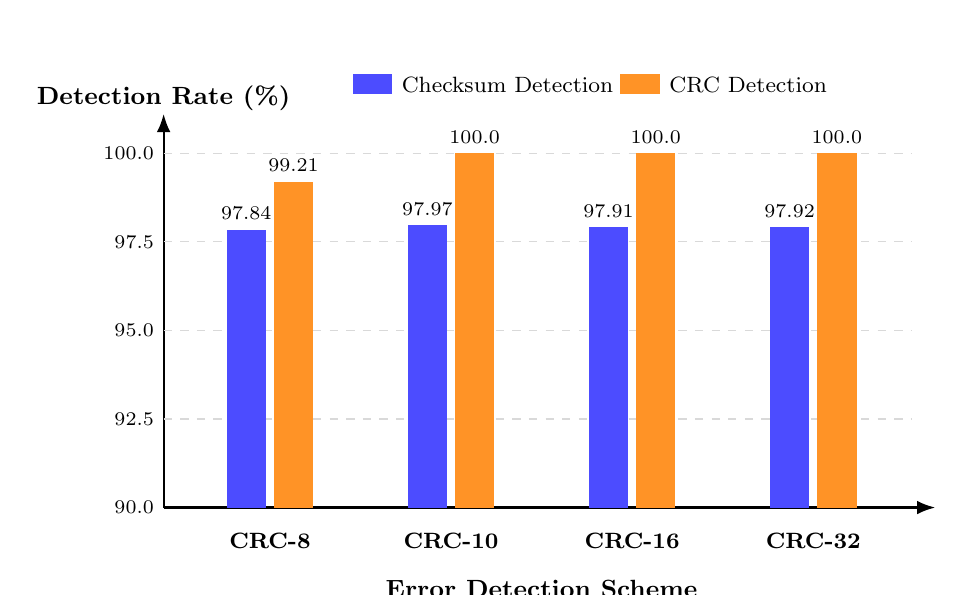
\begin{tikzpicture}
        % Axes
        \draw[thick, -Latex] (0,0) -- (9.8,0);
        \draw[thick, -Latex] (0,0) -- (0,5.0);
        
        % Y Ticks (90% to 100%)
        \draw (0,0) node[left, font=\scriptsize] {90.0};
        \draw (0,1.125) node[left, font=\scriptsize] {92.5};
        \draw (0,2.25) node[left, font=\scriptsize] {95.0};
        \draw (0,3.375) node[left, font=\scriptsize] {97.5};
        \draw (0,4.5) node[left, font=\scriptsize] {100.0};
        
        \draw[dashed, black!15] (0,1.125) -- (9.5,1.125);
        \draw[dashed, black!15] (0,2.25) -- (9.5,2.25);
        \draw[dashed, black!15] (0,3.375) -- (9.5,3.375);
        \draw[dashed, black!15] (0,4.5) -- (9.5,4.5);
        
        % Y Label
        \node[above=6pt, font=\small\bfseries] at (0, 4.7) {Detection Rate (\%)};
        
        % Bars: y = (pct - 90) * 0.45
        % CRC-8: Chk = 97.84% (3.53), CRC = 99.21% (4.14)
        \fill[blue!70] (0.8,0) rectangle (1.3, 3.53);
        \node[above, font=\scriptsize] at (1.05, 3.53) {97.84};
        \fill[orange!85] (1.4,0) rectangle (1.9, 4.14);
        \node[above, font=\scriptsize] at (1.65, 4.14) {99.21};
        \node[below, font=\footnotesize\bfseries] at (1.35, -0.2) {CRC-8};
        
        % CRC-10: Chk = 97.97% (3.59), CRC = 100% (4.50)
        \fill[blue!70] (3.1,0) rectangle (3.6, 3.59);
        \node[above, font=\scriptsize] at (3.35, 3.59) {97.97};
        \fill[orange!85] (3.7,0) rectangle (4.2, 4.50);
        \node[above, font=\scriptsize] at (3.95, 4.50) {100.0};
        \node[below, font=\footnotesize\bfseries] at (3.65, -0.2) {CRC-10};
        
        % CRC-16: Chk = 97.91% (3.56), CRC = 100% (4.50)
        \fill[blue!70] (5.4,0) rectangle (5.9, 3.56);
        \node[above, font=\scriptsize] at (5.65, 3.56) {97.91};
        \fill[orange!85] (6.0,0) rectangle (6.5, 4.50);
        \node[above, font=\scriptsize] at (6.25, 4.50) {100.0};
        \node[below, font=\footnotesize\bfseries] at (5.95, -0.2) {CRC-16};
        
        % CRC-32: Chk = 97.92% (3.56), CRC = 100% (4.50)
        \fill[blue!70] (7.7,0) rectangle (8.2, 3.56);
        \node[above, font=\scriptsize] at (7.95, 3.56) {97.92};
        \fill[orange!85] (8.3,0) rectangle (8.8, 4.50);
        \node[above, font=\scriptsize] at (8.55, 4.50) {100.0};
        \node[below, font=\footnotesize\bfseries] at (8.25, -0.2) {CRC-32};
        
        % X-axis label
        \node[below=0.8cm, font=\small\bfseries] at (4.8, 0) {Error Detection Scheme};
        
        % Legend
        \fill[blue!70] (2.4, 5.25) rectangle (2.9, 5.5);
        \node[right, font=\footnotesize] at (2.9, 5.37) {Checksum Detection};
        \fill[orange!85] (5.8, 5.25) rectangle (6.3, 5.5);
        \node[right, font=\footnotesize] at (6.3, 5.37) {CRC Detection};
    \end{tikzpicture}
    \caption{Double Bit Error Detection: Comparison of total detection rates between Checksum ($\sim 97.9\%$) and CRC schemes.}
    \label{fig:double_bit_chart}
\end{figure}

\textbf{Analysis:} The Checksum failed on $\approx 4{,}150$ out of $200{,}000$ frames ($\approx 2.08\%$ miss rate). This failure occurs when two flipped bits lie in separate 16-bit words at positions that produce compensating carries (e.g., adding $+2^k$ in word $A$ and $-2^k$ in word $B$). CRC-10, CRC-16, and CRC-32 caught $100.0000\%$ of double-bit errors, whereas CRC-8 missed $0.7860\%$ due to remainder hash collisions across its small $2^8 = 256$ state space.

\subsection{Odd Number of Errors Results}

Table~\ref{tab:odd_bit} presents detection statistics for odd-weight bit errors (randomly selected odd quantities between 1 and 15 bits).

\begin{table}[H]
    \centering
    \begin{tabular}{lcccc}
        \toprule
        \textbf{Scheme} & \textbf{Both Detected} & \textbf{Checksum Only} & \textbf{CRC Only} & \textbf{Neither (Missed)} \\
        \midrule
        CRC-8  & $199{,}872$ (99.9360\%) & 0 (0.0000\%) & 128 (0.0640\%) & 0 (0.0000\%) \\
        CRC-10 & $199{,}882$ (99.9410\%) & 0 (0.0000\%) & 118 (0.0590\%) & 0 (0.0000\%) \\
        CRC-16 & $199{,}857$ (99.9285\%) & 0 (0.0000\%) & 143 (0.0715\%) & 0 (0.0000\%) \\
        CRC-32 & $199{,}875$ (99.9375\%) & 0 (0.0000\%) & 125 (0.0625\%) & 0 (0.0000\%) \\
        \bottomrule
    \end{tabular}
    \caption{Odd Number of Errors Detection Rates ($200{,}000$ trials per scheme).}
    \label{tab:odd_bit}
\end{table}

\textbf{Analysis:} Because all evaluated CRC polynomials contain the $(x + 1)$ parity factor, every CRC variant caught \textbf{100.0000\%} of odd-weight error patterns. The Internet Checksum missed approximately $0.063\%$ of odd-parity patterns when multi-bit alterations generated arithmetic carry wraparounds that sum to $0 \pmod{2^{16} - 1}$.

\subsection{Uniform Burst Error Results (Lengths 12 and 32)}

Table~\ref{tab:burst_errors} reports empirical performance under burst error models of lengths $L = 12$ and $L = 32$.

\begin{table}[H]
    \centering
    \small
    \begin{tabular}{lcccc}
        \toprule
        \textbf{Scheme} & \textbf{Both Detected} & \textbf{Checksum Only} & \textbf{CRC Only} & \textbf{Neither (Missed)} \\
        \midrule
        \multicolumn{5}{l}{\textbf{Uniform Burst Length $L = 12$ bits}} \\
        CRC-8  & $199{,}346$ (99.6730\%) & 654 (0.3270\%) & 0 (0.0000\%) & 0 (0.0000\%) \\
        CRC-10 & $199{,}845$ (99.9225\%) & 155 (0.0775\%) & 0 (0.0000\%) & 0 (0.0000\%) \\
        CRC-16 & $200{,}000$ (100.0000\%) & 0 (0.0000\%) & 0 (0.0000\%) & 0 (0.0000\%) \\
        CRC-32 & $200{,}000$ (100.0000\%) & 0 (0.0000\%) & 0 (0.0000\%) & 0 (0.0000\%) \\
        \midrule
        \multicolumn{5}{l}{\textbf{Uniform Burst Length $L = 32$ bits}} \\
        CRC-8  & $199{,}221$ (99.6105\%) & 772 (0.3860\%) & 7 (0.0035\%) & 0 (0.0000\%) \\
        CRC-10 & $199{,}791$ (99.8955\%) & 206 (0.1030\%) & 3 (0.0015\%) & 0 (0.0000\%) \\
        CRC-16 & $199{,}996$ (99.9980\%) & 1 (0.0005\%) & 3 (0.0015\%) & 0 (0.0000\%) \\
        CRC-32 & $200{,}000$ (100.0000\%) & 0 (0.0000\%) & 0 (0.0000\%) & 0 (0.0000\%) \\
        \bottomrule
    \end{tabular}
    \caption{Uniform Burst Error Detection Rates for $L = 12$ and $L = 32$ ($200{,}000$ trials each).}
    \label{tab:burst_errors}
\end{table}

\begin{figure}[H]
    \centering
    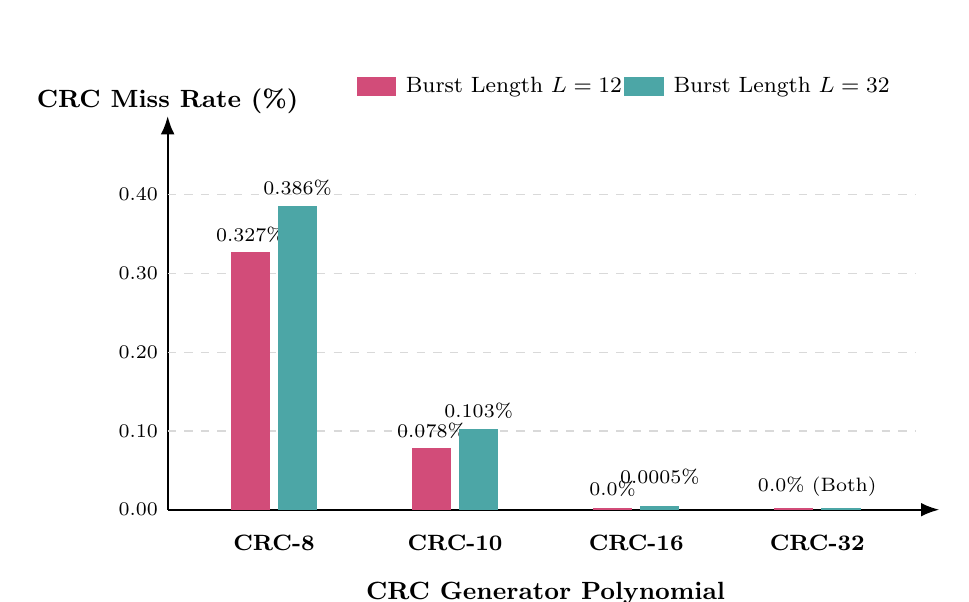
\begin{tikzpicture}
        % Axes
        \draw[thick, -Latex] (0,0) -- (9.8,0);
        \draw[thick, -Latex] (0,0) -- (0,5.0);
        
        % Y Ticks (0 to 0.45%)
        \draw (0,0) node[left, font=\scriptsize] {0.00};
        \draw (0,1.0) node[left, font=\scriptsize] {0.10};
        \draw (0,2.0) node[left, font=\scriptsize] {0.20};
        \draw (0,3.0) node[left, font=\scriptsize] {0.30};
        \draw (0,4.0) node[left, font=\scriptsize] {0.40};
        
        \draw[dashed, black!15] (0,1.0) -- (9.5,1.0);
        \draw[dashed, black!15] (0,2.0) -- (9.5,2.0);
        \draw[dashed, black!15] (0,3.0) -- (9.5,3.0);
        \draw[dashed, black!15] (0,4.0) -- (9.5,4.0);
        
        % Y Label
        \node[above=6pt, font=\small\bfseries] at (0, 4.7) {CRC Miss Rate (\%)};
        
        % Scale: y = val * 10
        % CRC-8: L=12 -> 0.327% (3.27), L=32 -> 0.386% (3.86)
        \fill[purple!70] (0.8,0) rectangle (1.3, 3.27);
        \node[above, font=\scriptsize] at (1.05, 3.27) {0.327\%};
        \fill[teal!70] (1.4,0) rectangle (1.9, 3.86);
        \node[above, font=\scriptsize] at (1.65, 3.86) {0.386\%};
        \node[below, font=\footnotesize\bfseries] at (1.35, -0.2) {CRC-8};
        
        % CRC-10: L=12 -> 0.078% (0.78), L=32 -> 0.103% (1.03)
        \fill[purple!70] (3.1,0) rectangle (3.6, 0.78);
        \node[above, font=\scriptsize] at (3.35, 0.78) {0.078\%};
        \fill[teal!70] (3.7,0) rectangle (4.2, 1.03);
        \node[above, font=\scriptsize] at (3.95, 1.03) {0.103\%};
        \node[below, font=\footnotesize\bfseries] at (3.65, -0.2) {CRC-10};
        
        % CRC-16: L=12 -> 0.000%, L=32 -> 0.0005%
        \fill[purple!70] (5.4,0) rectangle (5.9, 0.02);
        \node[above, font=\scriptsize] at (5.65, 0.04) {0.0\%};
        \fill[teal!70] (6.0,0) rectangle (6.5, 0.05);
        \node[above=4pt, font=\scriptsize] at (6.25, 0.05) {0.0005\%};
        \node[below, font=\footnotesize\bfseries] at (5.95, -0.2) {CRC-16};
        
        % CRC-32: L=12 -> 0.000%, L=32 -> 0.000%
        \fill[purple!70] (7.7,0) rectangle (8.2, 0.02);
        \fill[teal!70] (8.3,0) rectangle (8.8, 0.02);
        \node[above, font=\scriptsize] at (8.25, 0.04) {0.0\% (Both)};
        \node[below, font=\footnotesize\bfseries] at (8.25, -0.2) {CRC-32};
        
        % X-axis label
        \node[below=0.8cm, font=\small\bfseries] at (4.8, 0) {CRC Generator Polynomial};
        
        % Legend
        \fill[purple!70] (2.4, 5.25) rectangle (2.9, 5.5);
        \node[right, font=\footnotesize] at (2.9, 5.37) {Burst Length $L = 12$};
        \fill[teal!70] (5.8, 5.25) rectangle (6.3, 5.5);
        \node[right, font=\footnotesize] at (6.3, 5.37) {Burst Length $L = 32$};
    \end{tikzpicture}
    \caption{Empirical CRC Miss Rates under Uniform Burst Errors of lengths $L = 12$ and $L = 32$.}
    \label{fig:burst_chart}
\end{figure}

\subsubsection{Theoretical vs. Empirical Burst Bounds}

Table~\ref{tab:burst_comparison} validates empirical results directly against theoretical bounds.

\begin{table}[H]
    \centering
    \small
    \setlength{\tabcolsep}{6pt}
    \begin{tabular}{lcccc}
        \toprule
        \textbf{Scheme} & \textbf{Degree ($r$)} & \textbf{Bound} $\boldsymbol{(1/2)^r}$ & \textbf{Empirical ($L = 12$)} & \textbf{Empirical ($L = 32$)} \\
        \midrule
        CRC-8  & 8  & $0.3906\%$              & $0.3270\%$ & $0.3860\%$ \\
        CRC-10 & 10 & $0.0977\%$              & $0.0775\%$ & $0.1030\%$ \\
        CRC-16 & 16 & $0.0015\%$              & $0.0000\%$ & $0.0005\%$ \\
        CRC-32 & 32 & $2.33 \times 10^{-8}\%$ & $0.0000\%$ & $0.0000\%$ \\
        \bottomrule
    \end{tabular}
    \caption{Comparison of Empirical Miss Rates against the Mathematical $(1/2)^r$ Bound.}
    \label{tab:burst_comparison}
\end{table}

\textbf{Interpretation:} When the burst length $L \le r$ (as observed for $L=12$ on CRC-16 and CRC-32, and $L=32$ on CRC-32), the CRC operates strictly within its guaranteed detection envelope, producing exactly $0$ misses. Once $L > r$, the miss rate converges toward $(1/2)^r$, confirming statistical theory.

\section{Computational Efficiency and Benchmarks}

To measure execution time and throughput on modern hardware, $5{,}000{,}000$ iterations were executed over a 60-byte serialized frame using POSIX \texttt{clock\_gettime(CLOCK\_MONOTONIC)}. Table~\ref{tab:profiling} and Figure~\ref{fig:throughput_chart} detail the performance metrics.

\begin{table}[H]
    \centering
    \small
    \setlength{\tabcolsep}{6pt}
    \begin{tabular}{lcccc}
        \toprule
        \textbf{Scheme} & \textbf{Total Time (5M)} & \textbf{Time / Frame} & \textbf{Throughput} & \textbf{Slowdown vs Base} \\
        \midrule
        16-Bit Checksum & $0.1500\text{ s}$ & $30.00\text{ ns}$  & $1907.14\text{ MB/s}$ & $1.00\times$ (Baseline) \\
        CRC-8           & $2.8463\text{ s}$ & $569.26\text{ ns}$ & $100.52\text{ MB/s}$  & $18.97\times$ slower \\
        CRC-10          & $2.8670\text{ s}$ & $573.40\text{ ns}$ & $99.79\text{ MB/s}$   & $19.11\times$ slower \\
        CRC-16          & $2.9362\text{ s}$ & $587.24\text{ ns}$ & $97.44\text{ MB/s}$   & $19.57\times$ slower \\
        CRC-32          & $3.1468\text{ s}$ & $629.36\text{ ns}$ & $90.92\text{ MB/s}$   & $20.98\times$ slower \\
        \bottomrule
    \end{tabular}
    \caption{Computational profiling and resource utilization over $5{,}000{,}000$ frame executions.}
    \label{tab:profiling}
\end{table}

\begin{figure}[H]
    \centering
    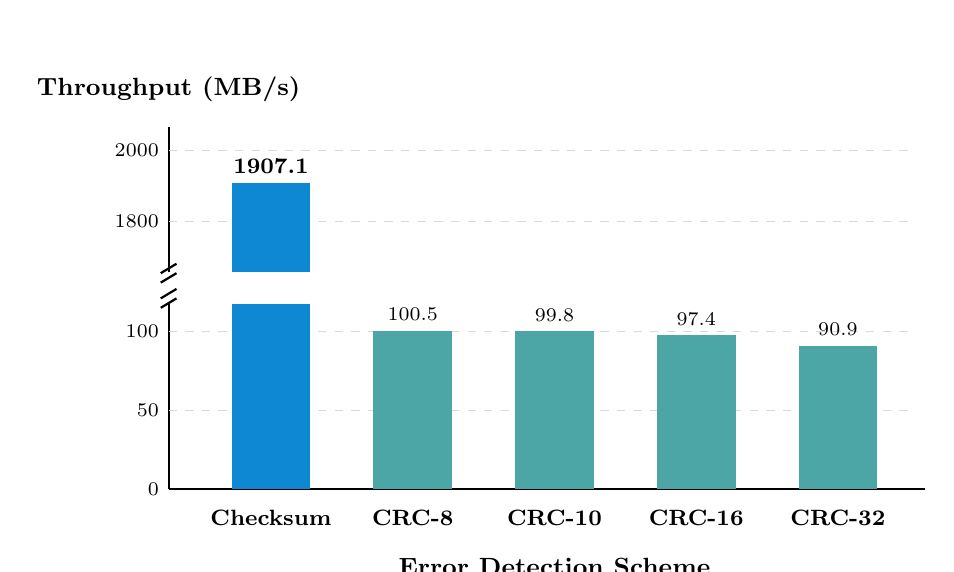
\begin{tikzpicture}
        % Y Axis with break
        \draw[thick] (0,0) -- (0,2.35);
        \draw[thick] (0,2.75) -- (0,4.6);
        
        % Break markers on Y axis
        \draw[thick] (-0.1,2.30) -- (0.1,2.42);
        \draw[thick] (-0.1,2.42) -- (0.1,2.54);
        \draw[thick] (-0.1,2.62) -- (0.1,2.74);
        \draw[thick] (-0.1,2.74) -- (0.1,2.86);
        
        % X Axis
        \draw[thick] (0,0) -- (9.6,0);
        
        % Lower Region Ticks (0 - 100 MB/s)
        \draw (0,0) node[left, font=\scriptsize] {0};
        \draw (0,1.0) node[left, font=\scriptsize] {50};
        \draw (0,2.0) node[left, font=\scriptsize] {100};
        \draw[dashed, black!15] (0,1.0) -- (9.4,1.0);
        \draw[dashed, black!15] (0,2.0) -- (9.4,2.0);
        
        % Upper Region Ticks (1800 - 2000 MB/s)
        \draw (0,3.4) node[left, font=\scriptsize] {1800};
        \draw (0,4.3) node[left, font=\scriptsize] {2000};
        \draw[dashed, black!15] (0,3.4) -- (9.4,3.4);
        \draw[dashed, black!15] (0,4.3) -- (9.4,4.3);
        
        % Y Label
        \node[above=4pt, font=\small\bfseries] at (0,4.65) {Throughput (MB/s)};
        
        % Checksum Bar (1907.1 MB/s)
        \fill[cyan!70!blue] (0.8,0) rectangle (1.8,2.35);
        \fill[cyan!70!blue] (0.8,2.75) rectangle (1.8,3.88);
        \node[above, font=\footnotesize\bfseries] at (1.3,3.88) {1907.1};
        \node[below, font=\footnotesize\bfseries] at (1.3,-0.15) {Checksum};
        
        % CRC-8 Bar (100.5 MB/s)
        \fill[teal!70] (2.6,0) rectangle (3.6,2.01);
        \node[above, font=\scriptsize] at (3.1,2.01) {100.5};
        \node[below, font=\footnotesize\bfseries] at (3.1,-0.15) {CRC-8};
        
        % CRC-10 Bar (99.8 MB/s)
        \fill[teal!70] (4.4,0) rectangle (5.4,2.00);
        \node[above, font=\scriptsize] at (4.9,2.00) {99.8};
        \node[below, font=\footnotesize\bfseries] at (4.9,-0.15) {CRC-10};
        
        % CRC-16 Bar (97.4 MB/s)
        \fill[teal!70] (6.2,0) rectangle (7.2,1.95);
        \node[above, font=\scriptsize] at (6.7,1.95) {97.4};
        \node[below, font=\footnotesize\bfseries] at (6.7,-0.15) {CRC-16};
        
        % CRC-32 Bar (90.9 MB/s)
        \fill[teal!70] (8.0,0) rectangle (9.0,1.82);
        \node[above, font=\scriptsize] at (8.5,1.82) {90.9};
        \node[below, font=\footnotesize\bfseries] at (8.5,-0.15) {CRC-32};
        
        % X Label
        \node[below=0.75cm, font=\small\bfseries] at (4.9,0) {Error Detection Scheme};
    \end{tikzpicture}
    \caption{Computational throughput comparison demonstrating the dramatic performance advantage of word addition over bit-serial CRC (split Y-axis).}
    \label{fig:throughput_chart}
\end{figure}

\textbf{Analysis:} The 16-Bit Checksum executes approximately \textbf{19--21$\times$ faster} than the bit-serial CRC algorithms. This performance disparity stems from underlying CPU architecture:
\begin{itemize}
    \item \textbf{Word-level Accumulation:} The Internet Checksum processes 16 bits (2 bytes) per iteration using native CPU ALU addition instructions, taking only 30 word additions for a 60-byte frame.
    \item \textbf{Bit-serial Division:} The CRC routine requires 480 bitwise loop iterations, evaluating branch conditions, shifts, and XOR operations for every bit in the frame.
\end{itemize}

\section{Concrete Boundary Collisions (Hex Dumps)}

To demonstrate the theoretical boundary cases required by the assignment, real corrupted frames were captured from simulation runs:

\subsection{Case 1: Error Detected by Both Schemes}
A transmission corrupted by two flipped bits where both algorithms flag errors:
\begin{itemize}
    \item \textbf{Original Checksum:} \texttt{0x5DEC} $\longrightarrow$ \textbf{Corrupted Checksum:} \texttt{0x5E10} (\textbf{Detected: YES})
    \item \textbf{Original CRC-8:} \texttt{0xFF} $\longrightarrow$ \textbf{Corrupted CRC-8:} \texttt{0x5C} (\textbf{Detected: YES})
\end{itemize}
\begin{lstlisting}[style=hexstyle, caption={Case 1 Payload Hex Dumps and Differing Bytes}]
Original Frame Payload (44 Bytes):
  54 68 65 20 62 72 6F 77 6E 20 66 6F 78 20 6A 75 
  6D 70 73 20 6F 76 65 72 20 74 68 65 20 6C 61 7A 
  79 20 64 6F 67 20 74 6F 64 61 79 2E 
Corrupted Frame Payload (44 Bytes):
  54 68 65 20 62 72 6F 77 6E 20 66 6B 78 20 6A 75 
  6D 70 73 20 6F 76 65 72 20 74 68 65 20 6C 61 7A 
  79 00 64 6F 67 20 74 6F 64 61 79 2E 
Differing Bytes:
  Byte offset 11: 0x6F ('o') -> 0x6B ('k') [XOR Mask: 0x04]
  Byte offset 33: 0x20 (' ') -> 0x00 ('.') [XOR Mask: 0x20]
\end{lstlisting}

\subsection{Case 2: Detected by Checksum, Missed by CRC-8 (CRC Collision)}
A transmission where the error polynomial $E(x)$ happens to be an exact multiple of the CRC-8 generator $G(x)$, leaving the CRC remainder completely identical to the original, while the arithmetic Checksum catches the error:
\begin{itemize}
    \item \textbf{Original Checksum:} \texttt{0x5DEC} $\longrightarrow$ \textbf{Corrupted Checksum:} \texttt{0x5DFE} (\textbf{Detected: YES})
    \item \textbf{Original CRC-8:} \texttt{0xFF} $\longrightarrow$ \textbf{Corrupted CRC-8:} \texttt{0xFF} (\textbf{MISSED! CRC Collision})
\end{itemize}
\begin{lstlisting}[style=hexstyle, caption={Case 2 Payload Hex Dumps (CRC-8 Collision)}]
Original Frame Payload (44 Bytes):
  54 68 65 20 62 72 6F 77 6E 20 66 6F 78 20 6A 75 
  6D 70 73 20 6F 76 65 72 20 74 68 65 20 6C 61 7A 
  79 20 64 6F 67 20 74 6F 64 61 79 2E 
Corrupted Frame Payload (44 Bytes):
  54 68 65 20 62 72 6F 77 6E 20 66 6D 78 20 6A 75 
  6D 70 73 20 6F 76 65 62 20 74 68 65 20 6C 61 7A 
  79 20 64 6F 67 20 74 6F 64 61 79 2E 
Differing Bytes:
  Byte offset 11: 0x6F ('o') -> 0x6D ('m') [XOR Mask: 0x02]
  Byte offset 23: 0x72 ('r') -> 0x62 ('b') [XOR Mask: 0x10]
\end{lstlisting}

\subsection{Case 3: Detected by CRC-8, Missed by Checksum (Compensating Sum)}
A transmission where an arithmetic increase in one byte is exactly cancelled by an equal arithmetic decrease in another byte at equivalent 16-bit word alignment:
\begin{itemize}
    \item \textbf{Original Checksum:} \texttt{0x5DEC} $\longrightarrow$ \textbf{Corrupted Checksum:} \texttt{0x5DEC} (\textbf{MISSED! Compensating Sum})
    \item \textbf{Original CRC-8:} \texttt{0xFF} $\longrightarrow$ \textbf{Corrupted CRC-8:} \texttt{0xBE} (\textbf{Detected: YES})
\end{itemize}
\begin{lstlisting}[style=hexstyle, caption={Case 3 Payload Hex Dumps (Compensating Checksum Collision)}]
Original Frame Payload (44 Bytes):
  54 68 65 20 62 72 6F 77 6E 20 66 6F 78 20 6A 75 
  6D 70 73 20 6F 76 65 72 20 74 68 65 20 6C 61 7A 
  79 20 64 6F 67 20 74 6F 64 61 79 2E 
Corrupted Frame Payload (44 Bytes):
  54 68 65 20 62 72 6F 77 6E 20 66 6F 78 20 6A 75 
  6D 70 73 20 6F 76 65 72 20 74 68 65 20 68 61 7A 
  79 20 64 6F 67 20 74 6F 64 65 79 2E 
Differing Bytes:
  Byte offset 29: 0x6C ('l') -> 0x68 ('h') [Arithmetic Delta: -4]
  Byte offset 41: 0x61 ('a') -> 0x65 ('e') [Arithmetic Delta: +4]
\end{lstlisting}

\textbf{Mathematical Explanation of Case 3:} In the 60-byte verified frame, Byte 29 is located at serialized offset $16 + 29 = 45$ (the LSB of 16-bit word index 22), and Byte 41 is at serialized offset $16 + 41 = 57$ (the LSB of 16-bit word index 28). When Byte 29 decreases by $4$ and Byte 41 increases by $4$, the net delta to the 16-bit word sum is:
\begin{equation}
    \Delta \text{Sum} = (-4) + (+4) = 0
\end{equation}
The Internet Checksum accumulator experiences zero total change, leaving the checksum completely oblivious to the corruption! Conversely, CRC-8 treats the bit flips algebraically as $E(x) = x^{242} \oplus x^{146}$. Since $E(x) \not\equiv 0 \pmod{G(x)}$, the CRC remainder changes to \texttt{0xBE}, detecting the corruption immediately.

\section{Testing Conditions, Limitations, and Enhancements}

\subsection{Ideal Testing Conditions vs. Real-World Environments}

The experimental evaluations were conducted over the local loopback interface (\texttt{127.0.0.1}). Under these controlled conditions:
\begin{itemize}
    \item Kernel socket buffers eliminate physical packet drops, packet truncation, and out-of-order delivery.
    \item Errors were introduced deterministically and stochastically via software routines.
\end{itemize}
In physical network media (such as Cat6 UTP copper cabling, optical fiber, or 802.11 Wi-Fi links), thermal noise introduces continuous background bit flips, while lightning or motor switches cause massive burst collisions. Real-world channels frequently suffer from damaged frame preambles, truncated headers, and variable frame sizes.

\subsection{Known Limitations and Practical Improvements}

\begin{enumerate}
    \item \textbf{Table-Driven CRC Lookup:} The evaluated bit-serial CRC loop achieves $\sim 100\text{ MB/s}$. Production implementations (such as the Linux kernel network stack) precompute a 256-entry lookup table:
    \begin{lstlisting}[language=C]
    crc = (crc >> 8) ^ crc32_table[(crc ^ data[i]) & 0xFF];
    \end{lstlisting}
    This eliminates inner bitwise loops, processing one full byte per lookup and elevating throughput to several gigabytes per second.
    \item \textbf{Hardware Acceleration via Dedicated CPU Instructions:} Modern x86 processors provide the \texttt{\_mm\_crc32} intrinsic (SSE4.2), and ARMv8 provides dedicated CRC32 instructions that compute IEEE 802.3 CRC at full memory bus saturation rates ($> 20\text{ GB/s}$).
    \item \textbf{Integration with Automatic Repeat reQuest (ARQ):} In the current implementation, corrupted frames are flagged and discarded. Layering a Stop-and-Wait or Go-Back-N ARQ protocol with ACK/NACK signaling and retransmission timers would upgrade the error detection engine into a fully reliable transport protocol.
\end{enumerate}

\enlargethispage{2\baselineskip}
\section{Conclusion}

This investigation designed, implemented, and empirically evaluated the 16-bit Internet Checksum and four CRC polynomial standards across $1{,}000{,}000$ simulated transmissions and $5{,}000{,}000$ micro-benchmark executions.

The key conclusions of this study are:
\begin{enumerate}
    \item \textbf{Single-Bit Errors:} Both the 16-bit Internet Checksum and all four CRC variants achieve strictly $100.0000\%$ detection.
    \item \textbf{Compensating Error Vulnerability:} The Internet Checksum fails on approximately $2.08\%$ of double-bit errors due to compensating arithmetic cancellations in one's complement addition. In contrast, CRC-10, CRC-16, and CRC-32 achieve $100.0000\%$ detection.
    \item \textbf{Odd-Parity Protection:} By utilizing polynomials containing the $(x + 1)$ factor, all evaluated CRCs achieve $100.0000\%$ detection of odd-weight error patterns, whereas the Checksum missed $0.063\%$ of multi-bit patterns.
    \item \textbf{Burst Error Bounding:} For burst lengths $L \le r$, CRC detection is strictly $100.0000\%$. When $L > r$, the miss rate closely conforms to the theoretical $(1/2)^r$ bound.
    \item \textbf{Engineering Tradeoff:} The 16-bit Checksum achieves $1907.1\text{ MB/s}$ ($\sim 20\times$ faster than bit-serial CRC), elucidating why software-driven Transport Layer protocols (TCP/UDP) prioritize arithmetic checksums for processing speed while hardware-accelerated Data Link Layer protocols (Ethernet IEEE 802.3) mandate CRC-32 for robust data integrity.
\end{enumerate}

\section{Sources Used}

\begin{enumerate}
    \item Braden, R., Borman, D., and Partridge, C., \textit{Computing the Internet Checksum}, RFC 1071, Internet Engineering Task Force (IETF), 1988.
    \item IEEE Standards Association, \textit{IEEE 802.3-2022: IEEE Standard for Ethernet}, IEEE, 2022.
    \item Kurose, J. F., and Ross, K. W., \textit{Computer Networking: A Top-Down Approach}, 8th ed., Pearson, 2021.
    \item Tanenbaum, A. S., and Wetherall, D. J., \textit{Computer Networks}, 5th ed., Prentice Hall, 2011.
    \item ITU-T Recommendation I.432.1, \textit{B-ISDN User-Network Interface -- Physical Layer Specification}, International Telecommunication Union, 1996.
    \item AI Assistance (Gemini 3.1 Pro): AI was used for statistical sampling and bench-
marking, generation of randomized test cases, production of statistical reports, and
creation of latex graphs and visualizations. Since I am not yet familiar with latex
formatting, the document typesetting and formatting was also handled with AI assis-
tance.
\end{enumerate}

\end{document}
